 \documentclass[11pt, oneside,a4paper]{book}
\pagestyle{headings}


%=============================================================================

\usepackage{amsthm}
\usepackage{xspace}
\usepackage{float}
\usepackage{ifthen}
\usepackage{amsbsy}
\usepackage{amssymb}
\usepackage{balance}
\usepackage{booktabs}
\usepackage{graphicx}
\usepackage{rotating}
\usepackage{multirow}
\usepackage{needspace}
\usepackage{microtype}
\usepackage{bold-extra}
\usepackage{geometry}
\usepackage{varioref}
\usepackage{xcolor}
\usepackage{textcomp}
\usepackage{listings}
\usepackage[normalem]{ulem} %emphasize still italic
\usepackage{ucs}

% \usepackage[utf8]{inputenc}
% \usepackage[htt]{hyphenat}
\usepackage{times}
\usepackage{url}
\usepackage{alltt}
\usepackage{amsmath}
\usepackage{xfrac}
\usepackage{subfigure}
\usepackage{appendix}
\usepackage{stmaryrd}   % for the \shortuparrow
\usepackage[utopia]{quotchap}

\usepackage{setspace}

%allow to change space between lines
\renewcommand{\baselinestretch}{1.2} 

\usepackage[numbers, sort&compress]{natbib}
\usepackage{mdwlist}        % support for better spaced lists
% allows for temporary adjustment of side margins
\usepackage{chngpage}
\usepackage[normalem]{ulem} 

\usepackage{enumitem}
\usepackage{capt-of}
% constants

\newcounter{qcounter}

% commands
\newcommand{\n}{$\cdot$}
\newcommand{\y}{\checkmark}
\newcommand{\subscript}[1]{$_{\textrm{\footnotesize{#1}}}$}
\newcommand{\superscript}[1]{$^{\textrm{\footnotesize{#1}}}$}
\newcommand{\vertical}[1]{\raisebox{-4em}{\begin{sideways}{#1}\end{sideways}}}



\newboolean{showedits}
\setboolean{showedits}{true} % toggle to show or hide edits
\ifthenelse{\boolean{showedits}}
{
       \newcommand{\ugh}[1]{\textcolor{red}{\uwave{#1}}} % please rephrase
       \newcommand{\ins}[1]{\textcolor{blue}{\uline{#1}}} % please insert
       \newcommand{\del}[1]{\textcolor{red}{\sout{#1}}} % please delete
       \newcommand{\chg}[2]{\textcolor{red}{\sout{#1}}{\ra}\textcolor{blue}{\uline{#2}}} % please change   
	\newcommand\brs[1]{\nbc{BRS}{#1}{blue}}       
       \newcommand{\nbc}[3]{
 {\colorbox{#3}{\bfseries\sffamily\scriptsize\textcolor{white}{#1}}}
 {\textcolor{#3}{\sf\small$\blacktriangleright$\textit{#2}$\blacktriangleleft$}}}
 

}{
       \newcommand{\ugh}[1]{#1} % please rephrase
       \newcommand{\ins}[1]{#1} % please insert
       \newcommand{\del}[1]{} % please delete
       \newcommand{\chg}[2]{#2}
       \newcommand{\nbc}[3]{}
}

	\newcommand\ho[1]{\nbc{H.}{#1}{violet}}
	
% ============================================================================
% Put edit comments in a really ugly standout display

\usepackage{xcolor}
\usepackage[normalem]{ulem}
\newcommand{\ra}{$\rightarrow$}


% comments \nb{label}{color}{text}
\newboolean{showcomments}
\setboolean{showcomments}{true}
\ifthenelse{\boolean{showcomments}}
    {\newcommand{\nb}[3]{
        {\colorbox{#2}{\bfseries\sffamily\scriptsize\textcolor{white}{#1}}}
        {\textcolor{#2}{\sf\small$\blacktriangleright$\textit{#3}$\blacktriangleleft$}}}
     \newcommand{\version}{\emph{\scriptsize$-$Id$-$}}
%	 \newcommand{\ugh}[1]{\textcolor{red}{\uwave{#1}}} % please rephrase
%	 \newcommand{\ins}[1]{\textcolor{blue}{\uline{#1}}} % please insert
%	 \newcommand{\del}[1]{\textcolor{red}{\sout{#1}}} % please delete
%	 \newcommand{\chg}[2]{\textcolor{red}{\sout{#1}}{\ra}\textcolor{blue}{\uline{#2}}} % please change
	 \newcommand{\chk}[1]{\textcolor{ForestGreen}{#1}} % changed, please check
	}
    {\newcommand{\nb}[3]{}
     \newcommand{\version}{}
	\newcommand{\chk}[1]{} % changed, please check
	}

% ============================================================================
% Make quotes be italic
\renewenvironment{quote}
    {\list{}{\rightmargin\leftmargin}%
     \item\relax\begin{it}}
    {\end{it}\endlist}

\newcommand{\ttimes}{\ensuremath{\times}}

%=============================================================================

\newcommand{\needlines}[1]{\Needspace{#1\baselineskip}}

% source code
\usepackage{xcolor}
\usepackage{textcomp}
\usepackage{listings}
\definecolor{source}{gray}{0.9}
\lstset{
	language={},
	% characters
	tabsize=3,
	upquote=true,
	escapechar={!},
	keepspaces=true,
	breaklines=false,
	alsoletter={:},
	breakautoindent=true,
	columns=fullflexible,
	showstringspaces=false,
	basicstyle=\footnotesize\ttfamily,
	% background
	frame=single,
    framerule=0pt,
	backgroundcolor=\color{source},
	% numbering
	numbersep=5pt,
	numberstyle=\tiny,
	numberfirstline=true,
	% captioning
	captionpos=b,
	numberbychapter=false,
	% formatting (html)
	moredelim=[is][\textbf]{<b>}{</b>},
	moredelim=[is][\textit]{<i>}{</i>},
	moredelim=[is][\uline]{<u>}{</u>}}
\newcommand{\ct}{\lstinline[backgroundcolor=\color{white},basicstyle=\footnotesize\ttfamily]}
\newcommand{\lct}[1]{{\small\tt #1}}

% end of json listing

%----------------------------------------------------------------------------
% references
\newcommand{\tabref}[1]{\hyperref[{tab:#1}]{Table~\ref*{tab:#1}}}
\newcommand{\figref}[1]{\hyperref[{fig:#1}]{Figure~\ref*{fig:#1}}}
\newcommand{\secref}[1]{\hyperref[{sec:#1}]{Section~\ref*{sec:#1}}}
\newcommand{\lstref}[1]{\hyperref[{lst:#1}]{Listing~\ref*{lst:#1}}}
\newcommand{\charef}[1]{\hyperref[{cha:#1}]{Chapter~\ref*{cha:#1}}}
%----------------------------------------------------------------------------

% abbreviations
\tracingcolors 4
\setcounter{tocdepth}{3}
\setcounter{secnumdepth}{3}
\newcommand{\ie}{\emph{i.e.,}\xspace}
\newcommand{\eg}{\emph{e.g.,}\xspace}
\newcommand{\etc}{\emph{etc.}\xspace}
\newcommand{\etal}{\emph{et al.}\xspace}


\newcommand{\newevenside}{
	\ifthenelse{\isodd{\thepage}}{\newpage}{
	\newpage
        \phantom{placeholder} % doesn't appear on page
	\thispagestyle{empty} % if want no header/footer
	\newpage
	}
}

\def\stretchfactor{1}
\newcommand{\mychapter}[1]{\setstretch{1}
    \chapter{#1}\setstretch{\stretchfactor}}

%----------------------------------------------------------------------------
\newcommand{\lessSpace}{\vspace{-1em}}
\DeclareGraphicsExtensions{.pdf,.png}
\graphicspath{{images/}}
\newcommand{\fig}[4]{
	\begin{figure}[#1]
		\centering
		\includegraphics[width=#2\textwidth]{#3}
		\lessSpace
		\caption{\label{fig:#3}#4}
	\end{figure}}

% ===========================================================================

%:CONFIGURE THIS

\newcommand{\thesistitle}{Citation Search Engine}
\newcommand{\thesisauthor}{Aliya Ibragimova}
\newcommand{\thesisauthorOrigin}{University of Fribourg}
\newcommand{\thesisleiter}{Prof.\ Dr.\ Oscar Nierstrasz}
\newcommand{\thesisasst}{Mr. Haidar Osman, Mr. Boris Spasojevic}
\newcommand{\thesisurl}{http://scg.unibe.ch/}
\newcommand{\thesissubtitle}{Academic paper search engine}
\newcommand{\thesisdate}{2015}

% ===========================================================================

\usepackage[ colorlinks=true, urlcolor=black, linkcolor=black,
			citecolor=black, bookmarksnumbered=true, bookmarks=true,
			plainpages=false,
			pdftitle={\thesistitle}, pdfauthor={\thesisauthor},
			pdfsubject={\thesissubtitle}, pdfpagelabels]{hyperref}

\newcommand{\hrref}[2]{\hyperref}
% ===========================================================================
% ===========================================================================


% D O C U M E N T
% % % % % % % % % % % % % % % % % % % % % % % % % % % % % % % % % %
\begin{document}

% T I T L E
% % % % % % % % % % % % % % % % % % % % % % % % % % % % % % % % % %
\begin{titlepage}  
  \begin{center}  
  
  \begin{figure}[t]  
  \vspace*{-2cm}        % to move header logo at the top 
  \center{
\includegraphics[scale=0.2]{logos/MSc_quer.png}}
  \vspace{0.4in}     
  \end{figure}

    \thispagestyle{empty}
    
    {\bfseries\Huge \thesistitle \par
    \Large \vspace{0.1in} \thesissubtitle \par}

    \vspace{0.3in} 
    \LARGE{\textbf{Master Thesis} \\}
    \vspace{0.4in}

    %{\Large \thesisauthor \par \thesisauthorOrigin}
    
    \vspace{0.3in}
    {\Large Faculty of Natural Sciences\\
            University of Bern \par}
    \vspace{0.3in}
    {\Large January \thesisdate \par}
    \vspace{0.3in}
    %Leiter der Arbeit: \par
   {\Large \thesisleiter} \par
      {\Large \thesisasst} \par
   \vspace{0.1in}
    {\Large Software Composition Group \par Institut f\"{u}r Informatik und angewandte Mathematik \par University of Bern, Switzerland \par}
  

  \vspace{0.9in}
 
  % === Logos ==============================================     
  \begin{figure}[htp]
    \centering
    
\includegraphics[scale=0.30]{logos/UNI_Bern.png}\hfill
    
\includegraphics[scale=0.30]{logos/UNI_Neuenburg.png}\hfill
    
\includegraphics[scale=0.80]{logos/UNI_Fribourg.png}
  \end{figure}
  % === // Logos ===========================================    


  \end{center}

\end{titlepage}


% A B S T R A C T
% % % % % % % % % % % % % % % % % % % % % % % % % % % % % % % % % %
\chapter*{\centering Abstract}
\begin{quotation}
\noindent 
Nowadays the amount of documents in World Wide Web grows exponentially. Tools that can facilitate information retrieval present a particular interest in the modern world. A typical web search engine that search
for information in World Wide Web is a software system that performs full-text indexing without considering meta information. This paper is devoted to the design of the academic paper search engine that takes advantage of meta-information, specifically citations. It is believed that citation is a very concise statement describing the source it refers to. Retrieving such statements can be particularly useful in writing scientific papers, for example, to build up a good argument. \\
This paper describes implementation of Citation Search Engine, a system that makes an attempt to automatically extract, index and aggregate citations from a set of scientific articles in PDF format. Besides it analyses the results of the deployment of the system on the collection of scientific papers provided by Software Composition Group.

\end{quotation}
\clearpage


% C O N T E N T S 
% % % % % % % % % % % % % % % % % % % % % % % % % % % % % % % % % % % % % % % %
\tableofcontents

%%%%%%%%%%%%%%%%%%%%%%%%%%%%%%%%%%
%%%% NEW CHAPTER %%%%%%%%%%%%%%%%%%%%%
%%%%%%%%%%%%%%%%%%%%%%%%%%%%%%%%%%
\chapter{Introduction}
\label{cha:introduction}

\section{Thesis statement}
We believe that considering meta information helps to build enhanced search systems that can facilitate information retrieval. Particularly, we target information retrieval for scientific papers. We consider citations as important text blocks summarising or judging previous scientific findings assisting in creating a new scientific work. We propose Citation Search Engine a software system that extracts citations from scientific papers, aggregates citations based on the referred source, then indexes extracted content. It provides a practical web interface that allows users to search for citations. 

\section{Goals}
We set following goals:
\begin{itemize}
	\item Introduce the state of the art techniques in information search.
	\item Explore the structure of scientific articles, reveal common patterns
	\item Design and implement the academic search engine.
	\item Deploy the system on the given collection of scientific papers
	\item Analyse results, define future work
\end{itemize}

\section{Outline}
The rest of the paper structured as follows:
\begin{description}
	\item[Chapter 1] The chapter gives an overview of a typical web search engine and shortly reviews popular academic search engines. 
	\item[Chapter 2] Devoted to the exploring the structure of scientific papers and identifying parsing challenges.
	\item[Chapter 3] Describes the desig and implementation of Citation Search Engine. 
	\item[Chapter 4] The chapter describes the deployment process and analysis the result of setting up the system on the given collection of scientific articles.
	\item[Chapter 5] Contains conclusion and possible future work. 
\end{description}

\chapter {Related Work}
\section{Typical web search engine}
Figure \ref{fig:web-search} illustrates a high level architecture of a standard web engine. It consist of three main components:
\begin{itemize}
\item Web Crawler
\item Data indexer
\item Search interface
\end{itemize} 

  \begin{figure}[htp]
    \centering
    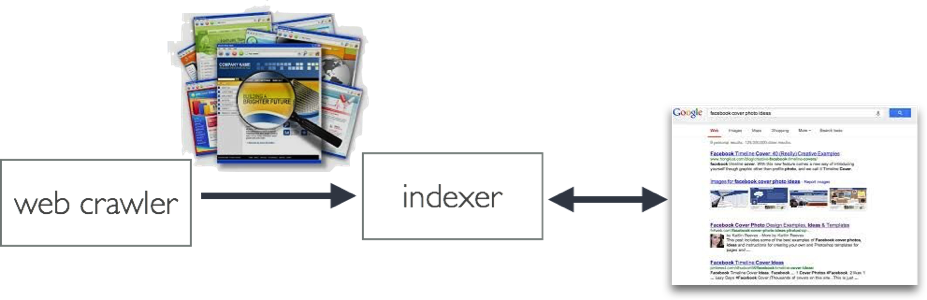
\includegraphics{web-search-engine}
    \caption{A high-level architecture of a typical web search engine}
    \label{fig:web-search}
  \end{figure}

\textbf{Web Crawler} is a program that browses the World Wide Web reading the content of web pages in order to provide up-to-date data to \textbf{Data Indexer}. Data Indexer decides how a page content should be stored in an index database. Index helps to quickly query information. Users can search and view query results through \textbf{Search Interface}. When a user makes a query a search engine analysis its index and returns best matched web pages according to specific to indexer criterias. \\
Web crawlers that fetch web pages with the content in the same domain are called focused or topical crawlers. An example of focused crawlers are academic-focused crawlers that crawls academical documents. Such crawlers become components of the "focused" search engines. Next chapter reviews most popular academical search engines.  

\section{Popular academic search engines}
\textbf{CiteSeer} \\
\textbf{Google Scholar} \\
\textbf{Microsoft Academic Search}

\chapter{The Problem}
In which we understand what the problem is in detail.

\chapter {Citation Search Engine}
In which you describe your solution.

\section{Overview of Architecture}
\section{Components}
\section{Parser -Challenges}

\chapter {The Validation}
In which you show how well the solution works.

\chapter {Conclusion and Future Work}
In which we step back, have a critical look at the entire work, then conclude, and learn what lays beyond this thesis.

%%CS can be used as a search engine for the repository of scientific papers in research institutes, in universities, or in any
%%organization that deals with collection of scientific papers. /Users/aliya/Documents/Master Thesis/template/scgbib/LatexTemplates/msc-thesis/preamble.tex



%END Doc
%-------------------------------------------------------

\bibliography{thesis}
\bibliographystyle{plain}

\end{document}